% Options for packages loaded elsewhere
\PassOptionsToPackage{unicode}{hyperref}
\PassOptionsToPackage{hyphens}{url}
\PassOptionsToPackage{dvipsnames,svgnames,x11names}{xcolor}
%
\documentclass[
  letterpaper,
  DIV=11,
  numbers=noendperiod]{scrartcl}

\usepackage{amsmath,amssymb}
\usepackage{iftex}
\ifPDFTeX
  \usepackage[T1]{fontenc}
  \usepackage[utf8]{inputenc}
  \usepackage{textcomp} % provide euro and other symbols
\else % if luatex or xetex
  \usepackage{unicode-math}
  \defaultfontfeatures{Scale=MatchLowercase}
  \defaultfontfeatures[\rmfamily]{Ligatures=TeX,Scale=1}
\fi
\usepackage{lmodern}
\ifPDFTeX\else  
    % xetex/luatex font selection
\fi
% Use upquote if available, for straight quotes in verbatim environments
\IfFileExists{upquote.sty}{\usepackage{upquote}}{}
\IfFileExists{microtype.sty}{% use microtype if available
  \usepackage[]{microtype}
  \UseMicrotypeSet[protrusion]{basicmath} % disable protrusion for tt fonts
}{}
\makeatletter
\@ifundefined{KOMAClassName}{% if non-KOMA class
  \IfFileExists{parskip.sty}{%
    \usepackage{parskip}
  }{% else
    \setlength{\parindent}{0pt}
    \setlength{\parskip}{6pt plus 2pt minus 1pt}}
}{% if KOMA class
  \KOMAoptions{parskip=half}}
\makeatother
\usepackage{xcolor}
\usepackage[letterpaper, margin=0.3in]{geometry}
\setlength{\emergencystretch}{3em} % prevent overfull lines
\setcounter{secnumdepth}{5}
% Make \paragraph and \subparagraph free-standing
\makeatletter
\ifx\paragraph\undefined\else
  \let\oldparagraph\paragraph
  \renewcommand{\paragraph}{
    \@ifstar
      \xxxParagraphStar
      \xxxParagraphNoStar
  }
  \newcommand{\xxxParagraphStar}[1]{\oldparagraph*{#1}\mbox{}}
  \newcommand{\xxxParagraphNoStar}[1]{\oldparagraph{#1}\mbox{}}
\fi
\ifx\subparagraph\undefined\else
  \let\oldsubparagraph\subparagraph
  \renewcommand{\subparagraph}{
    \@ifstar
      \xxxSubParagraphStar
      \xxxSubParagraphNoStar
  }
  \newcommand{\xxxSubParagraphStar}[1]{\oldsubparagraph*{#1}\mbox{}}
  \newcommand{\xxxSubParagraphNoStar}[1]{\oldsubparagraph{#1}\mbox{}}
\fi
\makeatother

\usepackage{color}
\usepackage{fancyvrb}
\newcommand{\VerbBar}{|}
\newcommand{\VERB}{\Verb[commandchars=\\\{\}]}
\DefineVerbatimEnvironment{Highlighting}{Verbatim}{commandchars=\\\{\}}
% Add ',fontsize=\small' for more characters per line
\usepackage{framed}
\definecolor{shadecolor}{RGB}{241,243,245}
\newenvironment{Shaded}{\begin{snugshade}}{\end{snugshade}}
\newcommand{\AlertTok}[1]{\textcolor[rgb]{0.68,0.00,0.00}{#1}}
\newcommand{\AnnotationTok}[1]{\textcolor[rgb]{0.37,0.37,0.37}{#1}}
\newcommand{\AttributeTok}[1]{\textcolor[rgb]{0.40,0.45,0.13}{#1}}
\newcommand{\BaseNTok}[1]{\textcolor[rgb]{0.68,0.00,0.00}{#1}}
\newcommand{\BuiltInTok}[1]{\textcolor[rgb]{0.00,0.23,0.31}{#1}}
\newcommand{\CharTok}[1]{\textcolor[rgb]{0.13,0.47,0.30}{#1}}
\newcommand{\CommentTok}[1]{\textcolor[rgb]{0.37,0.37,0.37}{#1}}
\newcommand{\CommentVarTok}[1]{\textcolor[rgb]{0.37,0.37,0.37}{\textit{#1}}}
\newcommand{\ConstantTok}[1]{\textcolor[rgb]{0.56,0.35,0.01}{#1}}
\newcommand{\ControlFlowTok}[1]{\textcolor[rgb]{0.00,0.23,0.31}{\textbf{#1}}}
\newcommand{\DataTypeTok}[1]{\textcolor[rgb]{0.68,0.00,0.00}{#1}}
\newcommand{\DecValTok}[1]{\textcolor[rgb]{0.68,0.00,0.00}{#1}}
\newcommand{\DocumentationTok}[1]{\textcolor[rgb]{0.37,0.37,0.37}{\textit{#1}}}
\newcommand{\ErrorTok}[1]{\textcolor[rgb]{0.68,0.00,0.00}{#1}}
\newcommand{\ExtensionTok}[1]{\textcolor[rgb]{0.00,0.23,0.31}{#1}}
\newcommand{\FloatTok}[1]{\textcolor[rgb]{0.68,0.00,0.00}{#1}}
\newcommand{\FunctionTok}[1]{\textcolor[rgb]{0.28,0.35,0.67}{#1}}
\newcommand{\ImportTok}[1]{\textcolor[rgb]{0.00,0.46,0.62}{#1}}
\newcommand{\InformationTok}[1]{\textcolor[rgb]{0.37,0.37,0.37}{#1}}
\newcommand{\KeywordTok}[1]{\textcolor[rgb]{0.00,0.23,0.31}{\textbf{#1}}}
\newcommand{\NormalTok}[1]{\textcolor[rgb]{0.00,0.23,0.31}{#1}}
\newcommand{\OperatorTok}[1]{\textcolor[rgb]{0.37,0.37,0.37}{#1}}
\newcommand{\OtherTok}[1]{\textcolor[rgb]{0.00,0.23,0.31}{#1}}
\newcommand{\PreprocessorTok}[1]{\textcolor[rgb]{0.68,0.00,0.00}{#1}}
\newcommand{\RegionMarkerTok}[1]{\textcolor[rgb]{0.00,0.23,0.31}{#1}}
\newcommand{\SpecialCharTok}[1]{\textcolor[rgb]{0.37,0.37,0.37}{#1}}
\newcommand{\SpecialStringTok}[1]{\textcolor[rgb]{0.13,0.47,0.30}{#1}}
\newcommand{\StringTok}[1]{\textcolor[rgb]{0.13,0.47,0.30}{#1}}
\newcommand{\VariableTok}[1]{\textcolor[rgb]{0.07,0.07,0.07}{#1}}
\newcommand{\VerbatimStringTok}[1]{\textcolor[rgb]{0.13,0.47,0.30}{#1}}
\newcommand{\WarningTok}[1]{\textcolor[rgb]{0.37,0.37,0.37}{\textit{#1}}}

\providecommand{\tightlist}{%
  \setlength{\itemsep}{0pt}\setlength{\parskip}{0pt}}\usepackage{longtable,booktabs,array}
\usepackage{calc} % for calculating minipage widths
% Correct order of tables after \paragraph or \subparagraph
\usepackage{etoolbox}
\makeatletter
\patchcmd\longtable{\par}{\if@noskipsec\mbox{}\fi\par}{}{}
\makeatother
% Allow footnotes in longtable head/foot
\IfFileExists{footnotehyper.sty}{\usepackage{footnotehyper}}{\usepackage{footnote}}
\makesavenoteenv{longtable}
\usepackage{graphicx}
\makeatletter
\def\maxwidth{\ifdim\Gin@nat@width>\linewidth\linewidth\else\Gin@nat@width\fi}
\def\maxheight{\ifdim\Gin@nat@height>\textheight\textheight\else\Gin@nat@height\fi}
\makeatother
% Scale images if necessary, so that they will not overflow the page
% margins by default, and it is still possible to overwrite the defaults
% using explicit options in \includegraphics[width, height, ...]{}
\setkeys{Gin}{width=\maxwidth,height=\maxheight,keepaspectratio}
% Set default figure placement to htbp
\makeatletter
\def\fps@figure{htbp}
\makeatother

\KOMAoption{captions}{tableheading}
\makeatletter
\@ifpackageloaded{tcolorbox}{}{\usepackage[skins,breakable]{tcolorbox}}
\@ifpackageloaded{fontawesome5}{}{\usepackage{fontawesome5}}
\definecolor{quarto-callout-color}{HTML}{909090}
\definecolor{quarto-callout-note-color}{HTML}{0758E5}
\definecolor{quarto-callout-important-color}{HTML}{CC1914}
\definecolor{quarto-callout-warning-color}{HTML}{EB9113}
\definecolor{quarto-callout-tip-color}{HTML}{00A047}
\definecolor{quarto-callout-caution-color}{HTML}{FC5300}
\definecolor{quarto-callout-color-frame}{HTML}{acacac}
\definecolor{quarto-callout-note-color-frame}{HTML}{4582ec}
\definecolor{quarto-callout-important-color-frame}{HTML}{d9534f}
\definecolor{quarto-callout-warning-color-frame}{HTML}{f0ad4e}
\definecolor{quarto-callout-tip-color-frame}{HTML}{02b875}
\definecolor{quarto-callout-caution-color-frame}{HTML}{fd7e14}
\makeatother
\makeatletter
\@ifpackageloaded{caption}{}{\usepackage{caption}}
\AtBeginDocument{%
\ifdefined\contentsname
  \renewcommand*\contentsname{Table of contents}
\else
  \newcommand\contentsname{Table of contents}
\fi
\ifdefined\listfigurename
  \renewcommand*\listfigurename{List of Figures}
\else
  \newcommand\listfigurename{List of Figures}
\fi
\ifdefined\listtablename
  \renewcommand*\listtablename{List of Tables}
\else
  \newcommand\listtablename{List of Tables}
\fi
\ifdefined\figurename
  \renewcommand*\figurename{Figure}
\else
  \newcommand\figurename{Figure}
\fi
\ifdefined\tablename
  \renewcommand*\tablename{Table}
\else
  \newcommand\tablename{Table}
\fi
}
\@ifpackageloaded{float}{}{\usepackage{float}}
\floatstyle{ruled}
\@ifundefined{c@chapter}{\newfloat{codelisting}{h}{lop}}{\newfloat{codelisting}{h}{lop}[chapter]}
\floatname{codelisting}{Listing}
\newcommand*\listoflistings{\listof{codelisting}{List of Listings}}
\makeatother
\makeatletter
\makeatother
\makeatletter
\@ifpackageloaded{caption}{}{\usepackage{caption}}
\@ifpackageloaded{subcaption}{}{\usepackage{subcaption}}
\makeatother

\ifLuaTeX
  \usepackage{selnolig}  % disable illegal ligatures
\fi
\usepackage{bookmark}

\IfFileExists{xurl.sty}{\usepackage{xurl}}{} % add URL line breaks if available
\urlstyle{same} % disable monospaced font for URLs
\hypersetup{
  pdftitle={Final Project - Step 2 (15 Points)},
  colorlinks=true,
  linkcolor={blue},
  filecolor={Maroon},
  citecolor={Blue},
  urlcolor={Blue},
  pdfcreator={LaTeX via pandoc}}


\title{Final Project - Step 2 (15 Points)}
\usepackage{etoolbox}
\makeatletter
\providecommand{\subtitle}[1]{% add subtitle to \maketitle
  \apptocmd{\@title}{\par {\large #1 \par}}{}{}
}
\makeatother
\subtitle{PSTAT100: Data Science Concepts and Analysis}
\author{}
\date{}

\begin{document}
\maketitle


\begin{tcolorbox}[enhanced jigsaw, left=2mm, breakable, colframe=quarto-callout-color-frame, leftrule=.75mm, toprule=.15mm, opacityback=0, colback=white, arc=.35mm, rightrule=.15mm, bottomrule=.15mm]

{\textbf{STUDENT NAME}}

\begin{itemize}
\tightlist
\item
  Valerie De La Fuente (valeriedelafuente)
\item
  Matthew Arteaga (matthewarteaga)
\item
  Phuc Lu (pdlu)
\item
  William Nelson (williamnelson)
\item
  Hayden Galletta (haydengalletta)
\end{itemize}

\end{tcolorbox}

\begin{tcolorbox}[enhanced jigsaw, left=2mm, breakable, toptitle=1mm, leftrule=.75mm, toprule=.15mm, bottomtitle=1mm, opacityback=0, colback=white, titlerule=0mm, opacitybacktitle=0.6, arc=.35mm, title=\textcolor{quarto-callout-caution-color}{\faFire}\hspace{0.5em}{Due Date}, colframe=quarto-callout-caution-color-frame, bottomrule=.15mm, rightrule=.15mm, coltitle=black, colbacktitle=quarto-callout-caution-color!10!white]

The deadline for this step is \textbf{Friday, May 9, 2025}.

\end{tcolorbox}

\begin{tcolorbox}[enhanced jigsaw, left=2mm, breakable, toptitle=1mm, leftrule=.75mm, toprule=.15mm, bottomtitle=1mm, opacityback=0, colback=white, titlerule=0mm, opacitybacktitle=0.6, arc=.35mm, title=\textcolor{quarto-callout-tip-color}{\faLightbulb}\hspace{0.5em}{Instructions}, colframe=quarto-callout-tip-color-frame, bottomrule=.15mm, rightrule=.15mm, coltitle=black, colbacktitle=quarto-callout-tip-color!10!white]

In this step, you will develop clear research questions and hypotheses
based on your selected dataset, and conduct a thorough Exploratory Data
Analysis (EDA). This foundational work is crucial for guiding your
analysis in the following steps.

\end{tcolorbox}

\section{Step 2: Research Questions, Hypotheses, and Exploratory Data
Analysis
(EDA)}\label{step-2-research-questions-hypotheses-and-exploratory-data-analysis-eda}

\subsection{Research Questions}\label{research-questions}

\textbf{Question 1}

Do certain dietary habits coincide with an increased rate of depression
among students?

\textbf{Question 2}

Is there a correlation between the amount of sleep a student gets and
the proportion of them that are depressed?

\textbf{Question 3}

Does the presence (and magnitude) of certain stressors have an impact on
the rate at which students are depressed?

\subsection{Hypotheses}\label{hypotheses}

\textbf{Hypothesis 1}

Students with moderate to healthy dietary habits will have lower rates
of depression compared to students with unhealthy dietary habits.

\textbf{Hypothesis 2}

Students who average more sleep per night will have lower rates of
depression compared to students who average less.

\textbf{Hypothesis 3}

Students with the highest collective reported stressors
(\texttt{Academic\ Pressure\ +\ Work\ Pressure\ +\ Financial\ Stress})
will have higher rates of depression compared to students with lower
collective reported stressors.

\subsection{Exploratory Data Analysis
(EDA)}\label{exploratory-data-analysis-eda}

\subsubsection{Data Cleaning}\label{data-cleaning}

\paragraph{Viewing the Data}\label{viewing-the-data}

\begin{Shaded}
\begin{Highlighting}[numbers=left,,]
\CommentTok{\# Load necessary packages}
\FunctionTok{library}\NormalTok{(readr)}
\FunctionTok{library}\NormalTok{(tidyverse)}
\FunctionTok{library}\NormalTok{(naniar)}
\FunctionTok{library}\NormalTok{(janitor)}

\CommentTok{\# Load in the data}
\NormalTok{depression\_data }\OtherTok{\textless{}{-}} \FunctionTok{read.csv}\NormalTok{(}\StringTok{"data/student\_depression\_dataset.csv"}\NormalTok{)}

\CommentTok{\# View the dataset}
\FunctionTok{head}\NormalTok{(depression\_data)}
\end{Highlighting}
\end{Shaded}

\begin{verbatim}
  id Gender Age          City Profession Academic.Pressure Work.Pressure CGPA
1  2   Male  33 Visakhapatnam    Student                 5             0 8.97
2  8 Female  24     Bangalore    Student                 2             0 5.90
3 26   Male  31      Srinagar    Student                 3             0 7.03
4 30 Female  28      Varanasi    Student                 3             0 5.59
5 32 Female  25        Jaipur    Student                 4             0 8.13
6 33   Male  29          Pune    Student                 2             0 5.70
  Study.Satisfaction Job.Satisfaction      Sleep.Duration Dietary.Habits
1                  2                0         '5-6 hours'        Healthy
2                  5                0         '5-6 hours'       Moderate
3                  5                0 'Less than 5 hours'        Healthy
4                  2                0         '7-8 hours'       Moderate
5                  3                0         '5-6 hours'       Moderate
6                  3                0 'Less than 5 hours'        Healthy
   Degree Have.you.ever.had.suicidal.thoughts.. Work.Study.Hours
1 B.Pharm                                   Yes                3
2     BSc                                    No                3
3      BA                                    No                9
4     BCA                                   Yes                4
5  M.Tech                                   Yes                1
6     PhD                                    No                4
  Financial.Stress Family.History.of.Mental.Illness Depression
1              1.0                               No          1
2              2.0                              Yes          0
3              1.0                              Yes          0
4              5.0                              Yes          1
5              1.0                               No          0
6              1.0                               No          0
\end{verbatim}

\begin{Shaded}
\begin{Highlighting}[numbers=left,,]
\CommentTok{\# Examine the dimensions}
\FunctionTok{dim}\NormalTok{(depression\_data)}
\end{Highlighting}
\end{Shaded}

\begin{verbatim}
[1] 27901    18
\end{verbatim}

There are 27901 observations and 18 variables in this dataset. The list
of variables is as follows:

\begin{itemize}
\item
  \texttt{id}: A unique identifier assigned to each student record in
  the dataset.
\item
  \texttt{Gender}: The gender of the student (e.g., Male, Female,
  Other). This helps in analyzing gender-specific trends in mental
  health.
\item
  \texttt{Age}: The age of the student in years.
\item
  \texttt{City}: The city or region where the student resides, providing
  geographical context for the analysis.
\item
  \texttt{Profession}: The field of work or study of the student, which
  may offer insights into occupational or academic stress factors.
\item
  \texttt{Academic\ Pressure}: A measure indicating the level of
  pressure the student faces in academic settings. This could include
  stress from exams, assignments, and overall academic expectations.
\item
  \texttt{Work\ Pressure}: A measure of the pressure related to work or
  job responsibilities, relevant for students who are employed alongside
  their studies.
\item
  \texttt{CGPA}: The cumulative grade point average of the student,
  reflecting overall academic performance.
\item
  \texttt{Study\ Satisfaction}: An indicator of how satisfied the
  student is with their studies, which can correlate with mental
  well-being.
\item
  \texttt{Job\ Satisfaction}: A measure of the student's satisfaction
  with their job or work environment, if applicable.
\item
  \texttt{Sleep\ Duration}: The average number of hours the student
  sleeps per day, which is an important factor in mental health.
\item
  \texttt{Dietary\ Habits}: An assessment of the student's eating
  patterns and nutritional habits, potentially impacting overall health
  and mood.
\item
  \texttt{Degree}: The academic degree or program that the student is
  pursuing.
\item
  \texttt{Have\ you\ ever\ had\ suicidal\ thoughts?}: A binary indicator
  (Yes/No) that reflects whether the student has ever experienced
  suicidal ideation.
\item
  \texttt{Work/Study\ Hours}: The average number of hours per day the
  student dedicates to work or study, which can influence stress levels.
\item
  \texttt{Financial\ Stress}: A measure of the stress experienced due to
  financial concerns, which may affect mental health.
\item
  \texttt{Family\ History\ of\ Mental\ Illness}: A measure of the stress
  experienced due to financial concerns, which may affect mental health.
\item
  \texttt{Depression}: The target variable that indicates whether the
  student is experiencing depression (Yes/No). This is the primary focus
  of the analysis.
\end{itemize}

\paragraph{Fixing Column Names}\label{fixing-column-names}

\begin{Shaded}
\begin{Highlighting}[numbers=left,,]
\CommentTok{\# Fix column names}
\NormalTok{depression\_data }\OtherTok{\textless{}{-}}\NormalTok{ depression\_data }\SpecialCharTok{\%\textgreater{}\%} 
  \FunctionTok{clean\_names}\NormalTok{() }\SpecialCharTok{\%\textgreater{}\%}
  \FunctionTok{rename}\NormalTok{(}
    \AttributeTok{cum\_gpa =}\NormalTok{ cgpa,}
    \AttributeTok{suicidal\_thoughts =}\NormalTok{ have\_you\_ever\_had\_suicidal\_thoughts,}
    \AttributeTok{fam\_mental\_illness =}\NormalTok{ family\_history\_of\_mental\_illness}
\NormalTok{  )}

\CommentTok{\# Check if names were fixed}
\FunctionTok{names}\NormalTok{(depression\_data)}
\end{Highlighting}
\end{Shaded}

\begin{verbatim}
 [1] "id"                 "gender"             "age"               
 [4] "city"               "profession"         "academic_pressure" 
 [7] "work_pressure"      "cum_gpa"            "study_satisfaction"
[10] "job_satisfaction"   "sleep_duration"     "dietary_habits"    
[13] "degree"             "suicidal_thoughts"  "work_study_hours"  
[16] "financial_stress"   "fam_mental_illness" "depression"        
\end{verbatim}

\paragraph{Missing Data}\label{missing-data}

\begin{Shaded}
\begin{Highlighting}[numbers=left,,]
\CommentTok{\# View missing data}
\FunctionTok{sum}\NormalTok{(}\FunctionTok{is.na}\NormalTok{(depression\_data))}
\end{Highlighting}
\end{Shaded}

\begin{verbatim}
[1] 0
\end{verbatim}

On the surface, there is no missing data. However, when looking at the
categories and their unique values, there are some signs of missingness.

For example, some categories have the \texttt{Other} category. Since
there is not way of figuring out what \texttt{Other} mean precisely, it
can be considered as an unknown category. To deal with this, it won't
remove but will still be concluded to not harm the data integrity.

Besides the other category, there is one variable that encodes its
missing value as \texttt{?}. This is a placeholder for missing value
under the \texttt{financial\ stress} variable. We'll deal with this by
encoding it as \texttt{NA}.

\begin{Shaded}
\begin{Highlighting}[numbers=left,,]
\CommentTok{\# Fixing the \textasciigrave{}financial\_stress\textasciigrave{} variable}
\NormalTok{depression\_data }\OtherTok{\textless{}{-}}\NormalTok{ depression\_data }\SpecialCharTok{\%\textgreater{}\%}
  \FunctionTok{mutate}\NormalTok{(}
    \AttributeTok{financial\_stress =} \FunctionTok{as.numeric}\NormalTok{(financial\_stress), }
    \CommentTok{\# convert string numbers to integers}
    \AttributeTok{financial\_stress =} \FunctionTok{case\_when}\NormalTok{(}
\NormalTok{      financial\_stress }\SpecialCharTok{==} \StringTok{"?"} \SpecialCharTok{\textasciitilde{}} \ConstantTok{NA}\NormalTok{,}
      \CommentTok{\# convert "?" to NA values}
      \AttributeTok{.default =}\NormalTok{ financial\_stress))}

\FunctionTok{sum}\NormalTok{(}\FunctionTok{is.na}\NormalTok{(depression\_data))}
\end{Highlighting}
\end{Shaded}

\begin{verbatim}
[1] 3
\end{verbatim}

Now, the total number of missing observation is 3, which comes from the
\texttt{financial\ stress} variable.

\begin{Shaded}
\begin{Highlighting}[numbers=left,,]
\FunctionTok{library}\NormalTok{(naniar)}
\NormalTok{depression\_data }\SpecialCharTok{\%\textgreater{}\%} \FunctionTok{vis\_miss}\NormalTok{()}
\end{Highlighting}
\end{Shaded}

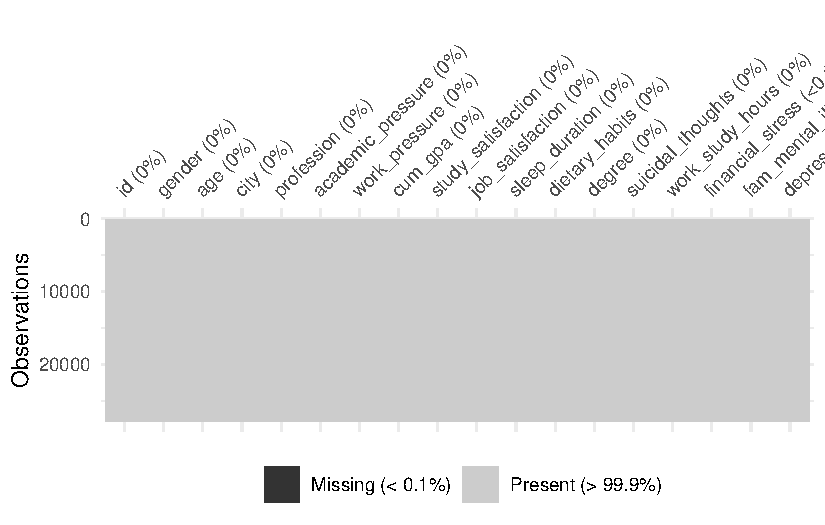
\includegraphics{Final_Project-Step-2_files/figure-pdf/unnamed-chunk-5-1.pdf}

This missingness only makes up \(\frac{3}{27,901}\) values or much less
than 0.1\% of the data set. We can simply remove these values without a
problem.

\begin{Shaded}
\begin{Highlighting}[numbers=left,,]
\NormalTok{depression\_data }\OtherTok{\textless{}{-}}\NormalTok{ depression\_data }\SpecialCharTok{\%\textgreater{}\%} \FunctionTok{na.omit}\NormalTok{()}
\NormalTok{depression\_data }\SpecialCharTok{\%\textgreater{}\%} \FunctionTok{dim}\NormalTok{()}
\end{Highlighting}
\end{Shaded}

\begin{verbatim}
[1] 27898    18
\end{verbatim}

\paragraph{Checking Data Types}\label{checking-data-types}

\begin{Shaded}
\begin{Highlighting}[numbers=left,,]
\CommentTok{\# Check data types of the variables}
\FunctionTok{str}\NormalTok{(depression\_data)}
\end{Highlighting}
\end{Shaded}

According to the output, we must mutate some variables. This includes
factorization and fixing some values that the variables take in.

\paragraph{Mutating Variables}\label{mutating-variables}

\begin{Shaded}
\begin{Highlighting}[numbers=left,,]
\CommentTok{\# Factorizing the \textasciigrave{}gender\textasciigrave{} variable}
\NormalTok{depression\_data}\SpecialCharTok{$}\NormalTok{gender }\OtherTok{\textless{}{-}} \FunctionTok{factor}\NormalTok{(depression\_data}\SpecialCharTok{$}\NormalTok{gender)}

\CommentTok{\# Fixing the \textasciigrave{}city\textasciigrave{} variable to change invalid entries}
\NormalTok{depression\_data }\OtherTok{\textless{}{-}}\NormalTok{ depression\_data }\SpecialCharTok{\%\textgreater{}\%}
  \FunctionTok{mutate}\NormalTok{(}\AttributeTok{city =} \FunctionTok{case\_when}\NormalTok{(}
\NormalTok{    city }\SpecialCharTok{==} \StringTok{"Khaziabad"} \SpecialCharTok{\textasciitilde{}} \StringTok{"Ghaziabad"}\NormalTok{,}
\NormalTok{    city }\SpecialCharTok{==} \StringTok{"Nalyan"} \SpecialCharTok{\textasciitilde{}} \StringTok{"Kalyan"}\NormalTok{,}
\NormalTok{    city }\SpecialCharTok{==} \StringTok{"\textquotesingle{}Less Delhi\textquotesingle{}"} \SpecialCharTok{\textasciitilde{}} \StringTok{"Delhi"}\NormalTok{,}
\NormalTok{    city }\SpecialCharTok{==} \StringTok{"\textquotesingle{}Less than 5 Kalyan\textquotesingle{}"} \SpecialCharTok{\textasciitilde{}} \StringTok{"Kalyan"}\NormalTok{,}
\NormalTok{    city }\SpecialCharTok{==} \StringTok{"3.0"} \SpecialCharTok{\textasciitilde{}} \StringTok{"Other"}\NormalTok{,}
\NormalTok{    city }\SpecialCharTok{==} \StringTok{"Saanvi"} \SpecialCharTok{\textasciitilde{}} \StringTok{"Other"}\NormalTok{,}
\NormalTok{    city }\SpecialCharTok{==} \StringTok{"M.Tech"} \SpecialCharTok{\textasciitilde{}} \StringTok{"Other"}\NormalTok{,}
\NormalTok{    city }\SpecialCharTok{==} \StringTok{"Bhavna"} \SpecialCharTok{\textasciitilde{}} \StringTok{"Other"}\NormalTok{,}
\NormalTok{    city }\SpecialCharTok{==} \StringTok{"City"} \SpecialCharTok{\textasciitilde{}} \StringTok{"Other"}\NormalTok{,}
\NormalTok{    city }\SpecialCharTok{==} \StringTok{"Mira"} \SpecialCharTok{\textasciitilde{}} \StringTok{"Other"}\NormalTok{,}
\NormalTok{    city }\SpecialCharTok{==} \StringTok{"Harsha"} \SpecialCharTok{\textasciitilde{}} \StringTok{"Other"}\NormalTok{,}
\NormalTok{    city }\SpecialCharTok{==} \StringTok{"Vaanya"} \SpecialCharTok{\textasciitilde{}} \StringTok{"Other"}\NormalTok{,}
\NormalTok{    city }\SpecialCharTok{==} \StringTok{"Gaurav"} \SpecialCharTok{\textasciitilde{}} \StringTok{"Other"}\NormalTok{,}
\NormalTok{    city }\SpecialCharTok{==} \StringTok{"Harsh"} \SpecialCharTok{\textasciitilde{}} \StringTok{"Other"}\NormalTok{,}
\NormalTok{    city }\SpecialCharTok{==} \StringTok{"Reyansh"} \SpecialCharTok{\textasciitilde{}} \StringTok{"Other"}\NormalTok{,}
\NormalTok{    city }\SpecialCharTok{==} \StringTok{"Kibara"} \SpecialCharTok{\textasciitilde{}} \StringTok{"Other"}\NormalTok{,}
\NormalTok{    city }\SpecialCharTok{==} \StringTok{"Rashi"} \SpecialCharTok{\textasciitilde{}} \StringTok{"Other"}\NormalTok{,}
\NormalTok{    city }\SpecialCharTok{==} \StringTok{"ME"} \SpecialCharTok{\textasciitilde{}} \StringTok{"Other"}\NormalTok{,}
\NormalTok{    city }\SpecialCharTok{==} \StringTok{"M.Com"} \SpecialCharTok{\textasciitilde{}} \StringTok{"Other"}\NormalTok{,}
\NormalTok{    city }\SpecialCharTok{==} \StringTok{"Mihir"} \SpecialCharTok{\textasciitilde{}} \StringTok{"Other"}\NormalTok{,}
\NormalTok{    city }\SpecialCharTok{==} \StringTok{"Nalini"} \SpecialCharTok{\textasciitilde{}} \StringTok{"Other"}\NormalTok{,}
\NormalTok{    city }\SpecialCharTok{==} \StringTok{"Nandini"} \SpecialCharTok{\textasciitilde{}} \StringTok{"Other"}\NormalTok{,}
    \ConstantTok{TRUE} \SpecialCharTok{\textasciitilde{}}\NormalTok{ city  }\CommentTok{\# Leave valid entries as they are}
\NormalTok{  ))}

\CommentTok{\# Fixing the \textasciigrave{}profession\textasciigrave{} variable to change invalid entries}
\NormalTok{depression\_data }\OtherTok{\textless{}{-}}\NormalTok{ depression\_data }\SpecialCharTok{\%\textgreater{}\%}
  \FunctionTok{mutate}\NormalTok{(}\AttributeTok{profession =} \FunctionTok{case\_when}\NormalTok{(}
\NormalTok{    profession }\SpecialCharTok{==} \StringTok{"\textquotesingle{}Civil Engineer\textquotesingle{}"} \SpecialCharTok{\textasciitilde{}} \StringTok{"Civil Engineer"}\NormalTok{,}
\NormalTok{    profession }\SpecialCharTok{==} \StringTok{"\textquotesingle{}UX/UI Designer\textquotesingle{}"} \SpecialCharTok{\textasciitilde{}} \StringTok{"UX/UI Designer"}\NormalTok{,}
\NormalTok{    profession }\SpecialCharTok{==} \StringTok{"\textquotesingle{}Digital Marketer\textquotesingle{}"} \SpecialCharTok{\textasciitilde{}} \StringTok{"Digital Marketer"}\NormalTok{,}
\NormalTok{    profession }\SpecialCharTok{==} \StringTok{"\textquotesingle{}Content Writer\textquotesingle{}"} \SpecialCharTok{\textasciitilde{}} \StringTok{"Content Writer"}\NormalTok{,}
\NormalTok{    profession }\SpecialCharTok{==} \StringTok{"\textquotesingle{}Educational Consultant\textquotesingle{}"} \SpecialCharTok{\textasciitilde{}} \StringTok{"Educational Consultant"}\NormalTok{,}
    \ConstantTok{TRUE} \SpecialCharTok{\textasciitilde{}}\NormalTok{ profession }\CommentTok{\# Leave valid entries as they are}
\NormalTok{  ))}

\CommentTok{\# Fixing the \textasciigrave{}sleep\_duration\textasciigrave{} variable to change invalid entries}
\NormalTok{depression\_data }\OtherTok{\textless{}{-}}\NormalTok{ depression\_data }\SpecialCharTok{\%\textgreater{}\%} 
  \FunctionTok{mutate}\NormalTok{(}\AttributeTok{sleep\_duration =} \FunctionTok{case\_when}\NormalTok{(}
\NormalTok{    sleep\_duration }\SpecialCharTok{==} \StringTok{"\textquotesingle{}5{-}6 hours\textquotesingle{}"} \SpecialCharTok{\textasciitilde{}} \StringTok{"5{-}6 hours"}\NormalTok{,}
\NormalTok{    sleep\_duration }\SpecialCharTok{==} \StringTok{"\textquotesingle{}Less than 5 hours\textquotesingle{}"} \SpecialCharTok{\textasciitilde{}} \StringTok{"Less than 5 hours"}\NormalTok{,}
\NormalTok{    sleep\_duration }\SpecialCharTok{==} \StringTok{"\textquotesingle{}7{-}8 hours\textquotesingle{}"} \SpecialCharTok{\textasciitilde{}} \StringTok{"7{-}8 hours"}\NormalTok{,}
\NormalTok{    sleep\_duration }\SpecialCharTok{==} \StringTok{"\textquotesingle{}More than 8 hours\textquotesingle{}"} \SpecialCharTok{\textasciitilde{}} \StringTok{"More than 8 hours"}\NormalTok{,}
\NormalTok{    sleep\_duration }\SpecialCharTok{==} \StringTok{"Others"} \SpecialCharTok{\textasciitilde{}} \StringTok{"Other"}
\NormalTok{  ))}

\CommentTok{\# Factorizing the \textasciigrave{}sleep\_duration\textasciigrave{} variable}
\NormalTok{depression\_data }\OtherTok{\textless{}{-}}\NormalTok{ depression\_data }\SpecialCharTok{\%\textgreater{}\%}
  \FunctionTok{mutate}\NormalTok{(}\AttributeTok{sleep\_duration =} \FunctionTok{factor}\NormalTok{(sleep\_duration, }
                                 \AttributeTok{levels =} \FunctionTok{c}\NormalTok{(}\StringTok{"Less than 5 hours"}\NormalTok{, }
                                            \StringTok{"5{-}6 hours"}\NormalTok{, }
                                            \StringTok{"7{-}8 hours"}\NormalTok{, }
                                            \StringTok{"More than 8 hours"}\NormalTok{, }
                                            \StringTok{"Other"}\NormalTok{),}
                                 \AttributeTok{ordered =} \ConstantTok{TRUE}\NormalTok{))}

\CommentTok{\# Fixing the \textasciigrave{}dietary\_habits\textasciigrave{} variable to change misspelling}
\NormalTok{depression\_data }\OtherTok{\textless{}{-}}\NormalTok{ depression\_data }\SpecialCharTok{\%\textgreater{}\%} 
  \FunctionTok{mutate}\NormalTok{(}\AttributeTok{dietary\_habits =} \FunctionTok{case\_when}\NormalTok{(}
\NormalTok{    dietary\_habits }\SpecialCharTok{==} \StringTok{"Others"} \SpecialCharTok{\textasciitilde{}} \StringTok{"Other"}\NormalTok{,}
    \ConstantTok{TRUE} \SpecialCharTok{\textasciitilde{}}\NormalTok{ dietary\_habits}
\NormalTok{  ))}

\CommentTok{\# Factorizing the \textasciigrave{}dietary\_habits\textasciigrave{} variable}
\NormalTok{depression\_data }\OtherTok{\textless{}{-}}\NormalTok{ depression\_data }\SpecialCharTok{\%\textgreater{}\%}
  \FunctionTok{mutate}\NormalTok{(}\AttributeTok{dietary\_habits =} \FunctionTok{factor}\NormalTok{(dietary\_habits,}
                                 \AttributeTok{levels =} \FunctionTok{c}\NormalTok{(}\StringTok{"Healthy"}\NormalTok{, }\StringTok{"Moderate"}\NormalTok{, }\StringTok{"Unhealthy"}\NormalTok{,}
                                            \StringTok{"Other"}\NormalTok{),}
                                 \AttributeTok{ordered =} \ConstantTok{TRUE}\NormalTok{))}

\CommentTok{\# Fixing the \textasciigrave{}degree\textasciigrave{} variable to change invalid entries}
\NormalTok{depression\_data }\OtherTok{\textless{}{-}}\NormalTok{ depression\_data }\SpecialCharTok{\%\textgreater{}\%}
  \FunctionTok{mutate}\NormalTok{(}\AttributeTok{degree =} \FunctionTok{case\_when}\NormalTok{(}
\NormalTok{    degree }\SpecialCharTok{==} \StringTok{"\textquotesingle{}Class 12\textquotesingle{}"} \SpecialCharTok{\textasciitilde{}} \StringTok{"Class 12"}\NormalTok{,}
\NormalTok{    degree }\SpecialCharTok{==} \StringTok{"Others"} \SpecialCharTok{\textasciitilde{}} \StringTok{"Other"}\NormalTok{,  }
    \CommentTok{\# Others could less than HS education or totally unknown. }
    \AttributeTok{.default =}\NormalTok{ degree}
\NormalTok{  ))}

\CommentTok{\# Factorizing the \textasciigrave{}suicidal\_thoughts\textasciigrave{} variable}
\NormalTok{depression\_data}\SpecialCharTok{$}\NormalTok{suicidal\_thoughts }\OtherTok{\textless{}{-}} \FunctionTok{factor}\NormalTok{(depression\_data}\SpecialCharTok{$}\NormalTok{suicidal\_thoughts)}

\CommentTok{\# Factorizing the \textasciigrave{}fam\_mental\_illness\textasciigrave{} variable}
\NormalTok{depression\_data}\SpecialCharTok{$}\NormalTok{fam\_mental\_illness }\OtherTok{\textless{}{-}} \FunctionTok{factor}\NormalTok{(depression\_data}\SpecialCharTok{$}\NormalTok{fam\_mental\_illness)}

\CommentTok{\# Turning the \textasciigrave{}depression\textasciigrave{} variable back to "yes" and "no" for visualization purposes}
\NormalTok{depression\_data }\OtherTok{\textless{}{-}}\NormalTok{ depression\_data }\SpecialCharTok{\%\textgreater{}\%} 
  \FunctionTok{mutate}\NormalTok{(}\AttributeTok{depression =} \FunctionTok{case\_when}\NormalTok{(}
\NormalTok{    depression }\SpecialCharTok{==} \DecValTok{0} \SpecialCharTok{\textasciitilde{}} \StringTok{"No"}\NormalTok{,}
\NormalTok{    depression }\SpecialCharTok{==} \DecValTok{1} \SpecialCharTok{\textasciitilde{}} \StringTok{"Yes"}
\NormalTok{  ))}

\CommentTok{\# Factorizing the \textasciigrave{}depression\textasciigrave{} variable}
\NormalTok{depression\_data}\SpecialCharTok{$}\NormalTok{depression }\OtherTok{\textless{}{-}} \FunctionTok{factor}\NormalTok{(depression\_data}\SpecialCharTok{$}\NormalTok{depression)}
\end{Highlighting}
\end{Shaded}

\begin{Shaded}
\begin{Highlighting}[numbers=left,,]
\CommentTok{\# Check data types of the variables again to ensure everything was properly done}
\FunctionTok{str}\NormalTok{(depression\_data)}
\end{Highlighting}
\end{Shaded}

According to the output, the data was successfully cleaned and the
variables are ready for visualization.

\subsection{Descriptive Statistics}\label{descriptive-statistics}

\subsubsection{Opinion Rating Variables}\label{opinion-rating-variables}

These are variables whose values were collected by asking the subjects
to rate their experience from a scale of 1-5. These include
\texttt{academic\ pressure}, \texttt{work\ pressure},
\texttt{study\ satisfaction}, \texttt{financial\ stress}. We chose to
isolate these to study their summary statistics because they're in a
different class compare to the other kind of numeric statistics. For
example, their values are bounded between 0 to 5 because that's the
range of the rating scale, where as age and cumulative GPA are not bound
to the same constraints.

\begin{Shaded}
\begin{Highlighting}[numbers=left,,]
\NormalTok{rating\_var }\OtherTok{\textless{}{-}}\NormalTok{ depression\_data }\SpecialCharTok{\%\textgreater{}\%} 
  \FunctionTok{select}\NormalTok{(academic\_pressure, work\_pressure, job\_satisfaction, study\_satisfaction, financial\_stress)}
\end{Highlighting}
\end{Shaded}

\begin{Shaded}
\begin{Highlighting}[numbers=left,,]
\NormalTok{rating\_var }\SpecialCharTok{\%\textgreater{}\%} \FunctionTok{summary}\NormalTok{()}
\end{Highlighting}
\end{Shaded}

\begin{longtable}[]{@{}
  >{\raggedright\arraybackslash}p{(\columnwidth - 10\tabcolsep) * \real{0.1667}}
  >{\raggedright\arraybackslash}p{(\columnwidth - 10\tabcolsep) * \real{0.1667}}
  >{\raggedright\arraybackslash}p{(\columnwidth - 10\tabcolsep) * \real{0.1667}}
  >{\raggedright\arraybackslash}p{(\columnwidth - 10\tabcolsep) * \real{0.1667}}
  >{\raggedright\arraybackslash}p{(\columnwidth - 10\tabcolsep) * \real{0.1667}}
  >{\raggedright\arraybackslash}p{(\columnwidth - 10\tabcolsep) * \real{0.1667}}@{}}
\toprule\noalign{}
\begin{minipage}[b]{\linewidth}\raggedright
Statistic
\end{minipage} & \begin{minipage}[b]{\linewidth}\raggedright
Academic Pressure
\end{minipage} & \begin{minipage}[b]{\linewidth}\raggedright
Work Pressure
\end{minipage} & \begin{minipage}[b]{\linewidth}\raggedright
Job Satisfaction
\end{minipage} & \begin{minipage}[b]{\linewidth}\raggedright
Study Satisfaction
\end{minipage} & \begin{minipage}[b]{\linewidth}\raggedright
Financial Stress
\end{minipage} \\
\midrule\noalign{}
\endhead
\bottomrule\noalign{}
\endlastfoot
Min. & 0.000 & 0.0000000 & 0.000000 & 0.000 & 1.00 \\
1st Qu. & 2.000 & 0.0000000 & 0.000000 & 2.000 & 2.00 \\
Median & 3.000 & 0.0000000 & 0.000000 & 3.000 & 3.00 \\
Mean & 3.141 & 0.0004300 & 0.000681 & 2.944 & 3.14 \\
3rd Qu. & 4.000 & 0.0000000 & 0.000000 & 4.000 & 4.00 \\
Max. & 5.000 & 5.0000000 & 4.000000 & 5.000 & 5.00 \\
\end{longtable}

A category that immediately jumps out is the extremely low overall
rating for \texttt{work\ pressure}. This means that the majority of
students in the data set reported that they have no pressure with their
work or job related responsibilities.

\begin{Shaded}
\begin{Highlighting}[numbers=left,,]
\CommentTok{\# table of work pressure and rating}
\NormalTok{depression\_data}\SpecialCharTok{$}\NormalTok{work\_pressure }\SpecialCharTok{\%\textgreater{}\%} \FunctionTok{table}\NormalTok{()}
\end{Highlighting}
\end{Shaded}

\begin{longtable}[]{@{}lllllll@{}}
\toprule\noalign{}
Work Pressure & 0 & 1 & 2 & 3 & 4 & 5 \\
\midrule\noalign{}
\endhead
\bottomrule\noalign{}
\endlastfoot
Frequency & 27710 & 0 & 1 & 0 & 0 & 2 \\
\end{longtable}

There are 2 students that reported 5 for work pressure. These are male
students from Rajkot and Chennai. They also share the same rating of 3
for financial stress, cumulative GPA of 0.0, they seem to be very
satisfied with their jobs with a rating of 4, no family history of
mental illness, and both have had high school education.

The one student who rated a 2 for work pressure is a male student from
from Lucknow, experiences academic pressure, 0.0 cumulative GPA, 1 for
job satisfaction, does have suicidal thoughts, 3 hours of work/study a
day, and does have family history of mental illness.

\texttt{Job\ satisfaction} is another category with the majority of
students express a rating of 0. For those with high job satisfaction, we
want to know what these type of people are and what they do.

\begin{Shaded}
\begin{Highlighting}[numbers=left,,]
\CommentTok{\# people with job satisfaction \textgreater{} 0}
\NormalTok{good\_job }\OtherTok{\textless{}{-}}\NormalTok{ depression\_data }\SpecialCharTok{\%\textgreater{}\%} \FunctionTok{filter}\NormalTok{(job\_satisfaction }\SpecialCharTok{\textgreater{}} \DecValTok{0}\NormalTok{)}
\end{Highlighting}
\end{Shaded}

There are 8 students in this data who rated themselves as having job
satisfaction greater than 0.

We're most interested in those who have the highest job satisfaction.

\begin{Shaded}
\begin{Highlighting}[numbers=left,,]
\NormalTok{good\_job }\SpecialCharTok{\%\textgreater{}\%} \FunctionTok{filter}\NormalTok{(job\_satisfaction }\SpecialCharTok{==} \FunctionTok{max}\NormalTok{(job\_satisfaction))}
\end{Highlighting}
\end{Shaded}

There are two male students in this data who rated their job
satisfaction a 4 which is higher than the majority of people in this
data set. Besides high job satisfaction, the other attributes that they
have in common are rated 3 for academic pressure, rated 3 for work
pressure, 0 study satisfaction, education up to grade 12, and no family
history of mental illness.

The first person is a 38 years old healthy male from Chennai, India.
This person sleeps for 5-6 hours, no suicidal thoughts, 2 hours of
work-study, rated a 3 for financial stress, and no depression.

The second person is an 18 years old moderately healthy male from
Rajkot. This person sleeps for 7-8 hours, does have suicidal thoughts, 9
hours of work-study, rated a 4 for financial stress, and does have
depression.

\begin{Shaded}
\begin{Highlighting}[numbers=left,,]
\NormalTok{depression\_data }\SpecialCharTok{\%\textgreater{}\%} 
  \FunctionTok{filter}\NormalTok{(work\_pressure }\SpecialCharTok{==} \FunctionTok{max}\NormalTok{(work\_pressure), }
\NormalTok{         job\_satisfaction }\SpecialCharTok{==} \FunctionTok{max}\NormalTok{(job\_satisfaction))}
\end{Highlighting}
\end{Shaded}

Between \texttt{work\ pressure} and \texttt{job\ satisfaction}, the two
students with the highest rating 5 for work pressure is also the person
with the highest job satisfaction with a rating of 4. They both have at
least high school education, 0 cumulative GPA, 0 study satisfaction, and
no family history of having a mental illness.

\subsubsection{Other Numeric Variables}\label{other-numeric-variables}

These variables include id, age, cumulative GPA and work/study hours.

\begin{Shaded}
\begin{Highlighting}[numbers=left,,]
\NormalTok{other\_numeric\_var }\OtherTok{\textless{}{-}}\NormalTok{ depression\_data }\SpecialCharTok{\%\textgreater{}\%} \FunctionTok{select\_if}\NormalTok{(is.numeric) }\SpecialCharTok{\%\textgreater{}\%} \FunctionTok{select}\NormalTok{(}\SpecialCharTok{{-}}\NormalTok{(rating\_var }\SpecialCharTok{\%\textgreater{}\%}\NormalTok{ colnames))}
\end{Highlighting}
\end{Shaded}

\begin{Shaded}
\begin{Highlighting}[numbers=left,,]
\NormalTok{other\_numeric\_var }\SpecialCharTok{\%\textgreater{}\%} \FunctionTok{summary}\NormalTok{()}
\end{Highlighting}
\end{Shaded}

\begin{longtable}[]{@{}lllll@{}}
\toprule\noalign{}
Statistic & ID & Age & Cumulative GPA & Work/Study Hours \\
\midrule\noalign{}
\endhead
\bottomrule\noalign{}
\endlastfoot
Min. & 2 & 18.0 & 0.000 & 0.000 \\
1st Qu. & 35053 & 21.0 & 6.290 & 4.000 \\
Median & 70694 & 25.0 & 7.770 & 8.000 \\
Mean & 70449 & 25.8 & 7.659 & 7.158 \\
3rd Qu. & 105828 & 30.0 & 8.920 & 10.000 \\
Max. & 140699 & 59.0 & 10.000 & 12.000 \\
\end{longtable}

\texttt{ID} can also be omitted from summary statistics because its
numeric value doesn't carry the same meaning as all of the other
variables. It's purpose is simply to provide a unique identity to each
observation.

The student with the oldest age in the data set is 59 years old and the
youngest student is 18 years old. On average, the students in the data
set tend to be 26 years old. Since the mean is slightly higher than the
median, this reveals that the shape of the distribution is slightly
right-skewed with tail. The age with the highest number of students is
24 and is followed at students who are 20 years old.

Since this data set was based in India, their GPA scale system is not
the same as the U.S. Instead of using the 4.0 scale, India's GPA scale
uses the 10.0 scale where it's out of 10. Under this system, the highest
GPA is 10.0 decreases from there. In this data set, the highest
cumulative GPA is 10.0 while the lowest is 0. The mean cumulative GPA is
7.656 or terms of the letter grade scale, it's approximately a B letter
grade.

There are 9 students who reported having a cumulative GPA of 0.0, which
is almost impossible to receive if they went to school. However, a
cumulative GPA of 0 is possible if the students had just started school.
Among these 9 students, the most shocking trait that they share is that
2/3 of them did express having suicidal thoughts and the majority of
them does not have education beyond high school.

For work or study hours, the max number is 12 hours can reflect
intensive work or academic schedules. On the other hand, the lowest
number of hour for work or study is 0, which means that these students
do not engage with work or study in a day. On average, the students tend
to work 7.158 hours. Since the middle of 0 to 12 is 6, but the mean and
median are above that, it can be inferred that students tend to a high
academic or work-related workload.

\subsubsection{Correlation Plot of Numeric
Variables}\label{correlation-plot-of-numeric-variables}

\begin{Shaded}
\begin{Highlighting}[numbers=left,,]
\FunctionTok{library}\NormalTok{(corrplot)}
\FunctionTok{cor}\NormalTok{(depression\_data }\SpecialCharTok{\%\textgreater{}\%} 
      \FunctionTok{select\_if}\NormalTok{(is.numeric)) }\SpecialCharTok{\%\textgreater{}\%} 
  \FunctionTok{corrplot}\NormalTok{(}\AttributeTok{type=}\StringTok{"lower"}\NormalTok{, }\AttributeTok{diag =} \ConstantTok{FALSE}\NormalTok{, }\AttributeTok{method =} \StringTok{"number"}\NormalTok{, }\AttributeTok{tl.srt =} \DecValTok{45}\NormalTok{)}
\end{Highlighting}
\end{Shaded}

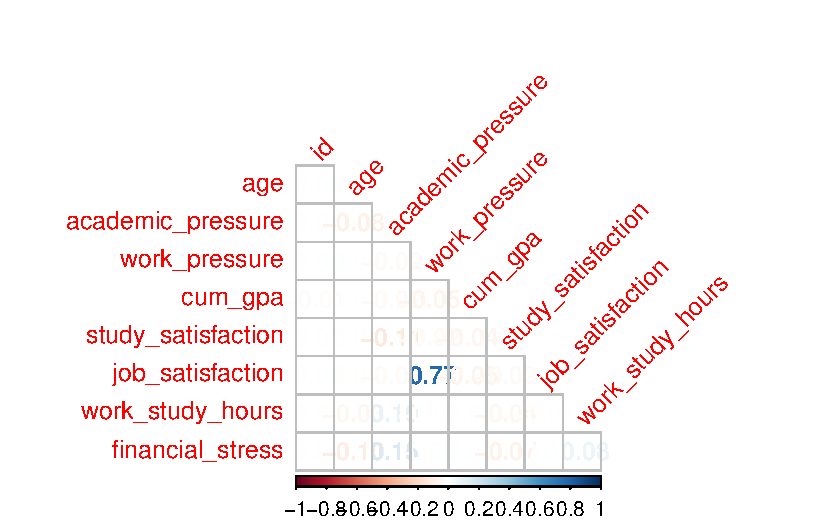
\includegraphics{Final_Project-Step-2_files/figure-pdf/unnamed-chunk-20-1.pdf}

There is a large correlation of 0.77 between the responses of
\texttt{Job\ Satisfaction} and \texttt{Work\ Pressure}. We should
explore this correlation:

\begin{Shaded}
\begin{Highlighting}[numbers=left,,]
\FunctionTok{table}\NormalTok{(depression\_data}\SpecialCharTok{$}\NormalTok{work\_pressure)}
\FunctionTok{table}\NormalTok{(depression\_data}\SpecialCharTok{$}\NormalTok{job\_satisfaction)}
\end{Highlighting}
\end{Shaded}

\begin{longtable}[]{@{}ll@{}}
\toprule\noalign{}
Work Pressure Level & Frequency \\
\midrule\noalign{}
\endhead
\bottomrule\noalign{}
\endlastfoot
0 & 27,895 \\
1 & 0 \\
2 & 1 \\
3 & 0 \\
4 & 0 \\
5 & 2 \\
\end{longtable}

\begin{longtable}[]{@{}ll@{}}
\toprule\noalign{}
Job Satisfaction Level & Frequency \\
\midrule\noalign{}
\endhead
\bottomrule\noalign{}
\endlastfoot
0 & 27,890 \\
1 & 2 \\
2 & 3 \\
3 & 1 \\
4 & 2 \\
\end{longtable}

When looking at the frequency table for \texttt{work\ pressure} and
\texttt{job\ satisfaction}, it is the case that nearly all of the
students expressed that they have the lowest level (0) in both
variables.The majority of students reported 0 in both variable could
also explain the high correlation. That is, if a student reported having
0 work pressure, it is also extremely likely that they will also report
having 0 job satisfaction. A reason for this probably because the
students do not have jobs and are full-time students.

\subsubsection{Binary Variables}\label{binary-variables}

Since these variables are continuous, it is better to analyze them by
comparing proportions of the two categories.

\paragraph{Depression}\label{depression}

\begin{Shaded}
\begin{Highlighting}[numbers=left,,]
\FunctionTok{round}\NormalTok{(}\FunctionTok{prop.table}\NormalTok{(}\FunctionTok{table}\NormalTok{(depression\_data}\SpecialCharTok{$}\NormalTok{depression)), }\AttributeTok{digits =} \DecValTok{3}\NormalTok{)}
\end{Highlighting}
\end{Shaded}

\begin{longtable}[]{@{}lll@{}}
\toprule\noalign{}
Depression & No & Yes \\
\midrule\noalign{}
\endhead
\bottomrule\noalign{}
\endlastfoot
Proportion & 0.414 & 0.586 \\
\end{longtable}

We see just below 60\% of students in the data set responded they
experience Depression. We proportion is not necessarily imbalanced, but
it's not totally balanced either. It's not necessary to be concern about
misrepresentation.

\paragraph{Suicidal Thoughts}\label{suicidal-thoughts}

\begin{Shaded}
\begin{Highlighting}[numbers=left,,]
\FunctionTok{round}\NormalTok{(}\FunctionTok{prop.table}\NormalTok{(}\FunctionTok{table}\NormalTok{(depression\_data}\SpecialCharTok{$}\NormalTok{suicidal\_thoughts)), }\AttributeTok{digits =} \DecValTok{3}\NormalTok{)}
\end{Highlighting}
\end{Shaded}

\begin{longtable}[]{@{}lll@{}}
\toprule\noalign{}
Suicidal Thoughts & No & Yes \\
\midrule\noalign{}
\endhead
\bottomrule\noalign{}
\endlastfoot
Proportion & 0.367 & 0.633 \\
\end{longtable}

We see 63.3\% of students respond they have had suicidal thoughts. This
means that there are more students who reported having suicidal thoughts
than those who did not. This proportion is imbalanced but it's doesn't
seem to be arbitrary. It would be interesting to explore the common
attributes among those who reported having suicidal thoughts. On the
other hand, the same thing could be done for those who reported not
having suicidal thoughts. Learning about the main indicator(s) for
suicidal thoughts or beneficial habits of those without suicidal
thoughts can potentially help students with suicidal thoughts later on
by incorporating the good habits into their lives.

\paragraph{Family Mental Illness}\label{family-mental-illness}

\begin{Shaded}
\begin{Highlighting}[numbers=left,,]
\FunctionTok{round}\NormalTok{(}\FunctionTok{prop.table}\NormalTok{(}\FunctionTok{table}\NormalTok{(depression\_data}\SpecialCharTok{$}\NormalTok{fam\_mental\_illness)), }\AttributeTok{digits =} \DecValTok{3}\NormalTok{)}
\end{Highlighting}
\end{Shaded}

\begin{longtable}[]{@{}lll@{}}
\toprule\noalign{}
Family History Mental Illness & No & Yes \\
\midrule\noalign{}
\endhead
\bottomrule\noalign{}
\endlastfoot
Proportion & 0.516 & 0.484 \\
\end{longtable}

It is nearly an even split between responses for the presence of mental
illness in the student's family, with a slightly higher frequency of
``No'' responses. Since both groups are fairly even, it could be
worthwhile to explore if having a family history of a mental illness
could potentially contribute to a student developing depression in their
lives.

\subsubsection{Categorical Variables}\label{categorical-variables}

These are variables with categories and numerical values to show how
many students fall under each category.

\paragraph{Dietary Habits}\label{dietary-habits}

\begin{Shaded}
\begin{Highlighting}[numbers=left,,]
\FunctionTok{round}\NormalTok{(}\FunctionTok{prop.table}\NormalTok{(}\FunctionTok{table}\NormalTok{(depression\_data}\SpecialCharTok{$}\NormalTok{dietary\_habits)), }\AttributeTok{digits =} \DecValTok{4}\NormalTok{)}
\end{Highlighting}
\end{Shaded}

\begin{longtable}[]{@{}lllll@{}}
\toprule\noalign{}
Dietary Habit & Healthy & Moderate & Unhealthy & Other \\
\midrule\noalign{}
\endhead
\bottomrule\noalign{}
\endlastfoot
Proportion & 0.2742 & 0.3556 & 0.3698 & 0.0004 \\
\end{longtable}

More students have moderate and unhealthy dietary habits than healthy
dietary habits. There is a very small amount of students reported having
a more nuanced dietary habit. It is difficult to tell what they eat, but
we decided to just leave this category be instead of removing it.

\paragraph{Sleep Duration}\label{sleep-duration}

\begin{Shaded}
\begin{Highlighting}[numbers=left,,]
\FunctionTok{round}\NormalTok{(}\FunctionTok{prop.table}\NormalTok{(}\FunctionTok{table}\NormalTok{(depression\_data}\SpecialCharTok{$}\NormalTok{sleep\_duration)), }\AttributeTok{digits =} \DecValTok{3}\NormalTok{)}
\end{Highlighting}
\end{Shaded}

\begin{longtable}[]{@{}
  >{\raggedright\arraybackslash}p{(\columnwidth - 10\tabcolsep) * \real{0.1928}}
  >{\raggedright\arraybackslash}p{(\columnwidth - 10\tabcolsep) * \real{0.2289}}
  >{\raggedright\arraybackslash}p{(\columnwidth - 10\tabcolsep) * \real{0.1325}}
  >{\raggedright\arraybackslash}p{(\columnwidth - 10\tabcolsep) * \real{0.1325}}
  >{\raggedright\arraybackslash}p{(\columnwidth - 10\tabcolsep) * \real{0.2289}}
  >{\raggedright\arraybackslash}p{(\columnwidth - 10\tabcolsep) * \real{0.0843}}@{}}
\toprule\noalign{}
\begin{minipage}[b]{\linewidth}\raggedright
Sleep Duration
\end{minipage} & \begin{minipage}[b]{\linewidth}\raggedright
Less than 5 hours
\end{minipage} & \begin{minipage}[b]{\linewidth}\raggedright
5-6 hours
\end{minipage} & \begin{minipage}[b]{\linewidth}\raggedright
7-8 hours
\end{minipage} & \begin{minipage}[b]{\linewidth}\raggedright
More than 8 hours
\end{minipage} & \begin{minipage}[b]{\linewidth}\raggedright
Other
\end{minipage} \\
\midrule\noalign{}
\endhead
\bottomrule\noalign{}
\endlastfoot
Proportion & 0.298 & 0.222 & 0.263 & 0.217 & 0.001 \\
\end{longtable}

We see that almost a third of students said they get less than 5 hours
of sleep on average. There is again, a small group of students who
report having a sleep duration that's different from the other
categories. They could have a very unstable sleeping habit that
fluctuates a lot every night. This category could be valuable for
looking into if having a regular sleep schedule as opposed to one that
fluctuates can contribute to having depression.

\subsection{Data Visualization}\label{data-visualization}

This first graph is a bar plot that helps to answer hypothesis 1 by
visualizing the correlation between a healthy diet and depression. The
results of this bar plot clearly indicate a strong correlation with a
unhealthy diet and rates of depression.

\begin{Shaded}
\begin{Highlighting}[numbers=left,,]
\CommentTok{\# For dietary habits}
\FunctionTok{ggplot}\NormalTok{(depression\_data, }\FunctionTok{aes}\NormalTok{(}\AttributeTok{x =}\NormalTok{ dietary\_habits, }\AttributeTok{fill =} \FunctionTok{factor}\NormalTok{(depression))) }\SpecialCharTok{+}
  \FunctionTok{geom\_bar}\NormalTok{(}\AttributeTok{position =} \StringTok{"fill"}\NormalTok{, }\AttributeTok{color =} \StringTok{"black"}\NormalTok{) }\SpecialCharTok{+}
  \FunctionTok{scale\_y\_continuous}\NormalTok{(}\AttributeTok{labels =}\NormalTok{ scales}\SpecialCharTok{::}\NormalTok{percent) }\SpecialCharTok{+}
  \FunctionTok{labs}\NormalTok{(}\AttributeTok{title =} \StringTok{"Depression Distribution by Dietary Habit"}\NormalTok{,}
       \AttributeTok{x =} \StringTok{"Dietary Habit"}\NormalTok{, }\AttributeTok{y =} \StringTok{"Proportion"}\NormalTok{,}
       \AttributeTok{fill =} \StringTok{"Depression"}\NormalTok{) }\SpecialCharTok{+}
  \FunctionTok{theme\_bw}\NormalTok{(}\AttributeTok{base\_size =} \DecValTok{12}\NormalTok{) }\SpecialCharTok{+}
  \FunctionTok{theme}\NormalTok{(}\AttributeTok{axis.text.x =} \FunctionTok{element\_text}\NormalTok{(}\AttributeTok{angle =} \DecValTok{45}\NormalTok{, }\AttributeTok{hjust =} \DecValTok{1}\NormalTok{))}
\end{Highlighting}
\end{Shaded}

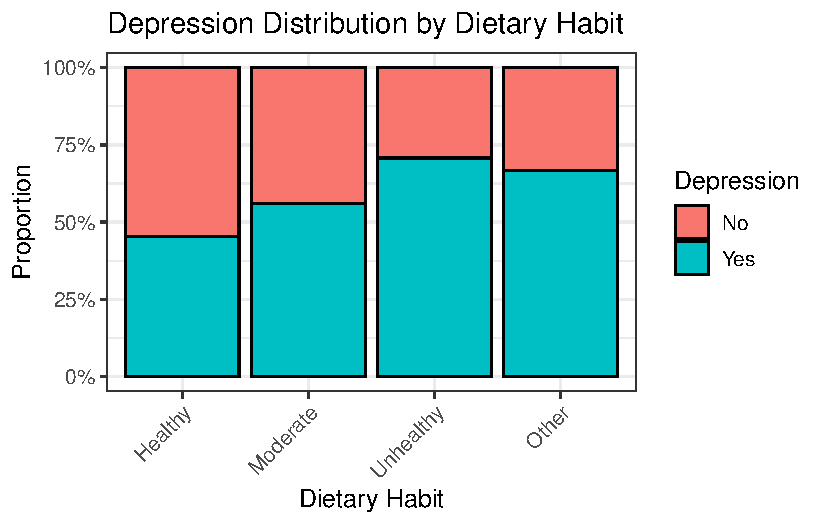
\includegraphics{Final_Project-Step-2_files/figure-pdf/unnamed-chunk-27-1.pdf}

The second graph is a bar plot that helps to answer hypothesis 2 by
visualizing the correlation between sleep patterns and depression. The
results of this bar plot seem to indicate that people getting less than
5 hours of sleep have a significantly higher rate of depression and
people who get more than 8 hours of sleep have a significantly lower
rate of depression.

\begin{Shaded}
\begin{Highlighting}[numbers=left,,]
\CommentTok{\# Convert \textquotesingle{}depression\textquotesingle{} factor to numeric: "No" = 0, "Yes" = 1}
\NormalTok{depression\_data }\OtherTok{\textless{}{-}}\NormalTok{ depression\_data }\SpecialCharTok{\%\textgreater{}\%}
  \FunctionTok{mutate}\NormalTok{(}\AttributeTok{depression\_numeric =} \FunctionTok{as.numeric}\NormalTok{(depression) }\SpecialCharTok{{-}} \DecValTok{1}\NormalTok{)}

\CommentTok{\# Create summarized depression rates and standard errors by sleep duration}
\NormalTok{sleep\_summary }\OtherTok{\textless{}{-}}\NormalTok{ depression\_data }\SpecialCharTok{\%\textgreater{}\%}
  \FunctionTok{group\_by}\NormalTok{(sleep\_duration) }\SpecialCharTok{\%\textgreater{}\%}
  \FunctionTok{summarise}\NormalTok{(}
    \AttributeTok{mean\_dep =} \FunctionTok{mean}\NormalTok{(depression\_numeric, }\AttributeTok{na.rm =} \ConstantTok{TRUE}\NormalTok{),}
    \AttributeTok{se =} \FunctionTok{sd}\NormalTok{(depression\_numeric, }\AttributeTok{na.rm =} \ConstantTok{TRUE}\NormalTok{) }\SpecialCharTok{/} \FunctionTok{sqrt}\NormalTok{(}\FunctionTok{n}\NormalTok{())}
\NormalTok{  )}

\CommentTok{\# Bar plot with error bars}
\FunctionTok{ggplot}\NormalTok{(sleep\_summary, }\FunctionTok{aes}\NormalTok{(}\AttributeTok{x =}\NormalTok{ sleep\_duration, }\AttributeTok{y =}\NormalTok{ mean\_dep, }\AttributeTok{fill =}\NormalTok{ sleep\_duration)) }\SpecialCharTok{+}
  \FunctionTok{geom\_col}\NormalTok{(}\AttributeTok{show.legend =} \ConstantTok{FALSE}\NormalTok{) }\SpecialCharTok{+}

  \FunctionTok{labs}\NormalTok{(}
    \AttributeTok{title =} \StringTok{"Depression Rate by Sleep Duration"}\NormalTok{,}
    \AttributeTok{x =} \StringTok{"Sleep Duration"}\NormalTok{,}
    \AttributeTok{y =} \StringTok{"Mean Depression Rate"}
\NormalTok{  ) }\SpecialCharTok{+}
  \FunctionTok{theme\_minimal}\NormalTok{(}\AttributeTok{base\_size =} \DecValTok{13}\NormalTok{) }\SpecialCharTok{+}
  \FunctionTok{theme}\NormalTok{(}\AttributeTok{axis.text.x =} \FunctionTok{element\_text}\NormalTok{(}\AttributeTok{angle =} \DecValTok{45}\NormalTok{, }\AttributeTok{hjust =} \DecValTok{1}\NormalTok{))}
\end{Highlighting}
\end{Shaded}

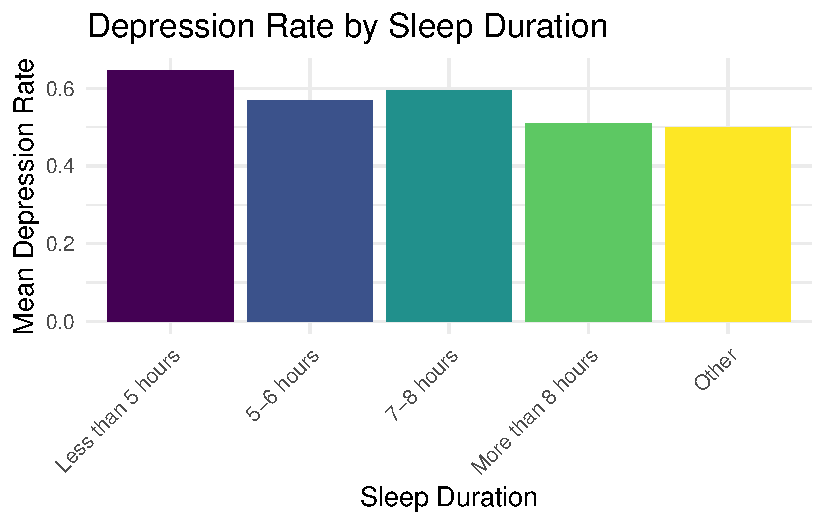
\includegraphics{Final_Project-Step-2_files/figure-pdf/unnamed-chunk-28-1.pdf}

This final graph is a boxplot that helps visualize hypothesis 3 and
shows the correlation between multiple stressor factors and depression.
The results seem to indicate a correlation with the total stressors and
depression.

\begin{Shaded}
\begin{Highlighting}[numbers=left,,]
\NormalTok{depression\_data}\SpecialCharTok{$}\NormalTok{financial\_stress }\OtherTok{\textless{}{-}} \FunctionTok{as.numeric}\NormalTok{(depression\_data}\SpecialCharTok{$}\NormalTok{financial\_stress)}
\NormalTok{depression\_data}\SpecialCharTok{$}\NormalTok{total\_stress }\OtherTok{\textless{}{-}}\NormalTok{ depression\_data}\SpecialCharTok{$}\NormalTok{academic\_pressure }\SpecialCharTok{+}
\NormalTok{                                 depression\_data}\SpecialCharTok{$}\NormalTok{work\_pressure }\SpecialCharTok{+}
\NormalTok{                                 depression\_data}\SpecialCharTok{$}\NormalTok{financial\_stress}

\FunctionTok{ggplot}\NormalTok{(depression\_data, }\FunctionTok{aes}\NormalTok{(}\AttributeTok{x =} \FunctionTok{factor}\NormalTok{(depression), }\AttributeTok{y =}\NormalTok{ total\_stress, }\AttributeTok{fill =} \FunctionTok{factor}\NormalTok{(depression))) }\SpecialCharTok{+}
  \FunctionTok{geom\_boxplot}\NormalTok{() }\SpecialCharTok{+}
  \FunctionTok{labs}\NormalTok{(}\AttributeTok{title =} \StringTok{"Total Reported Stress vs Depression"}\NormalTok{, }\AttributeTok{x =} \StringTok{"Depression (0 = No, 1 = Yes)"}\NormalTok{, }\AttributeTok{y =} \StringTok{"Total Stress"}\NormalTok{) }\SpecialCharTok{+}
  \FunctionTok{theme\_minimal}\NormalTok{()}
\end{Highlighting}
\end{Shaded}

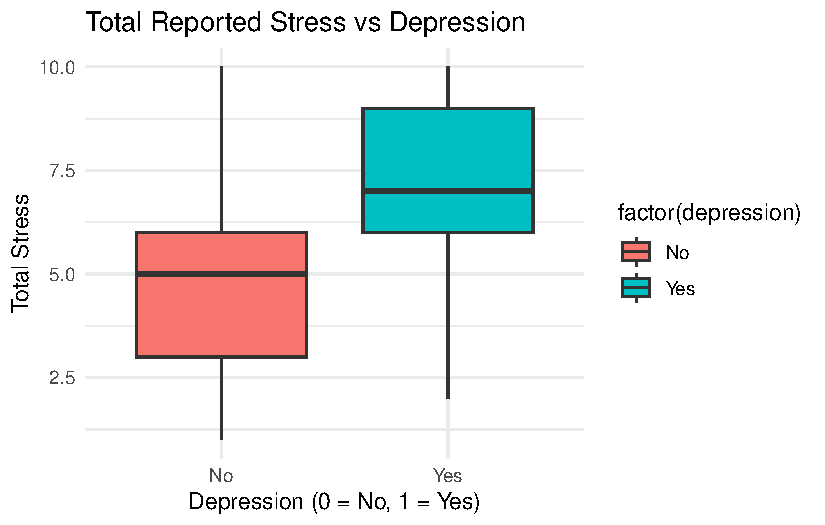
\includegraphics{Final_Project-Step-2_files/figure-pdf/unnamed-chunk-29-1.pdf}




\end{document}
